\documentclass[msc,pdftex]{coppe}
\usepackage[latin1]{inputenc}
\usepackage{amsmath,amssymb}

\makelosymbols
\makeloabbreviations

\begin{document}
  \title{Controle de Miss�o do Rob� DORIS}
  \foreigntitle{DORIS Mission Control}
  \author{Renan Salles}{de Freitas}
  \advisor{Prof.}{Ramon}{Romankevicius}{D.Sc.}
  \coadvisor{Prof.}{Pal}{From}{D.Sc.}
  \examiner{Prof.}{}{D.Sc.}
  \examiner{Prof.}{}{Ph.D.}
  \examiner{Prof.}{}{D.Sc.}
  \department{PEE}
  \date{03}{2015}
  \keyword{Controle de Miss�o}
  \keyword{Rede de Petri}
  \keyword{}
  \maketitle

  \frontmatter
  \dedication{� minha m�e pelo dom da vida e pelo amparo ao longo desses anos.\\
}


  \chapter*{Agradecimentos}




  \begin{abstract}



\end{abstract}


  \begin{foreignabstract}



\end{foreignabstract}


  \tableofcontents 
  \listoffigures
  \listoftables
  \printlosymbols
  \printloabbreviations

  \mainmatter
  \chapter{Introdu��o}

%Em m�todos num�ricos para obter solu��es aproximadas de equa��es diferenciais,
%tais como o m�todo dos elementos finitos (MEF)\abbrev{MEF}{m�todo de elementos
%finitos} e o m�todo dos volumes finitos (MVF)\abbrev{MVF}{m�todo de volumes
%finitos}, o dom�nio no qual estas equa��es foram definidas � discretizado em
%sub-dom�nios simples denominados \textit{elementos}.

%Denotemos o dom�nio por $\Omega$\symbl{$\Omega$}{dom�nio de defini��o de uma
%equa��o diferencial}. Seja $\partial \Omega$ o contorno de
%$\Omega$.\symbl{$\partial$}{operador do contorno.}

\section{Motiva�{\~ a}o}

\section{Objetivo}

\section{Metodologia}

\section{Organiza�{\~ a}o da tese}

  \chapter{Revis�o Bibliogr�fica}

Neste cap�tulo, s�o apresentados alguns fundamentos te�ricos necess�rios para o
entendimento desta disserta��o e alguns dos principais trabalhos e pesquisas
cient�ficas relacionados ao controle de miss�o de rob�s m�veis. O objetivo deste
levantamento bibliogr�fico � apresentar t�cnicas vi�veis e aplica��es de
diversos sistemas de controle de miss�o, e direcionar o leitor para os
conhecimentos aplicados no controle de miss�o do rob� DORIS, projeto que
envolve esta disserta��o. Os estudos ser�o apresentados de forma cronol�gica.

Em 1986, um dos primeiros estudos em controle de miss�o foi desenvolvido por
Rodney Brooks, em BROOKS, R.A. [1]. Este estudo � a base para diversos
trabalhos atuais que envolvem controle de miss�o de rob�s m�veis. Os
desafios de rob�s aut�nomos apontados por Brooks e que ainda ilustram os
problemas da atualidade s�o: \emph{m�ltiplos objetivos}, \emph{m�ltiplos
sensores}, \emph{robustez} e \emph{extensibilidade}. Esses desafios n�o s�o
suportados pela arquitetura tradicional de um sistema de controle, como ser�
visto adiante.

Os m�ltiplos objetivos de rob�s m�veis podem:
\begin{itemize}
  \item Ser conflitantes: por exemplo, um rob� pode estar tentando alcan�ar um
  determinado ponto no espa�o, por�m evitando obst�culos locais.
  \item Ter rela��es de prioridade: por exemplo, um rob� que inspeciona trilhos
  de tr�m deve sair dos trilhos ao ouvir o sinal de um tr�m chegando, mesmo se estiver
  finalizando a opera��o.
  \item Ser denpendentes: objetivos de \emph{alto n�vel} englobam diversos
  objetivos de \emph{baixo n�vel}. No caso do exemplo acima, o rob� que sai do
  trilho para evitar o tr�m deve se manter equilibrado para n�o cair. Outros
  artigos mais recentes, e que ser�o discutidos em outras subse��es, separam
  esses objetivos em \emph{tarefas} (objetivos de \emph{alto n�vel}) e
  \emph{primitivas do ve�culo}.
\end{itemize}

Os m�ltiplos sensores de um rob� m�vel dependem de sua aplica��o, por�m
normalmente ele � provido de in�meros sensores redundantes ou que s�o utilizados
para uma mesma tarefa. Por exemplo, a utiliza��o de encoders para odometria e
localiza��o, e c�meras que comparam quadros j� coletados previamente tamb�m para
localiza��o. Os sensores podem apresentar erros ou resultados conflitantes,
portanto a fus�o da informa��o de m�ltiplos sensores, a determina��o de seus
graus de confiabilidade e onde devem ser considerados s�o decis�es que
o rob� deve saber fazer.

Um rob� deve ser robusto. Quando um sensor falha, o rob� deve se
adaptar e utilizar os outros sensores que ainda funcionam para realizar as
tarefas. Quando o ambiente sofre altera��es, o rob� deve ser capaz de cumprir
determinadas fun��es essenciais.

A extensabilidade constitui em acrescentar mais sensores e,
portanto, aumentar a capacidade do rob�, este pode executar novas tarefas.
Por�m, isso vai esbarrar com a limita��o de processamento do rob�.

A modelagem de rob�s de acordo com suas principais funcionalidades e o
desenvolvimento de novas arquiteturas para seus controles s�o o �mago no estudo
de controle de miss�o de rob�s m�veis. Brooks prop�e uma
nova arquitetura, como pode ser visto na figura~\ref{BROOKS_1}. O autor
comenta que essa decomposi��o conduz a uma arquitetura radicalmente diferente para sistema de
controle de rob�s m�veis, com diferen�as radicais em estrat�gias de
implementa��o a n�vel de hardware e com grandes vantagens em robustez,
constru��o e teste.

\begin{figure}[H]
\centering
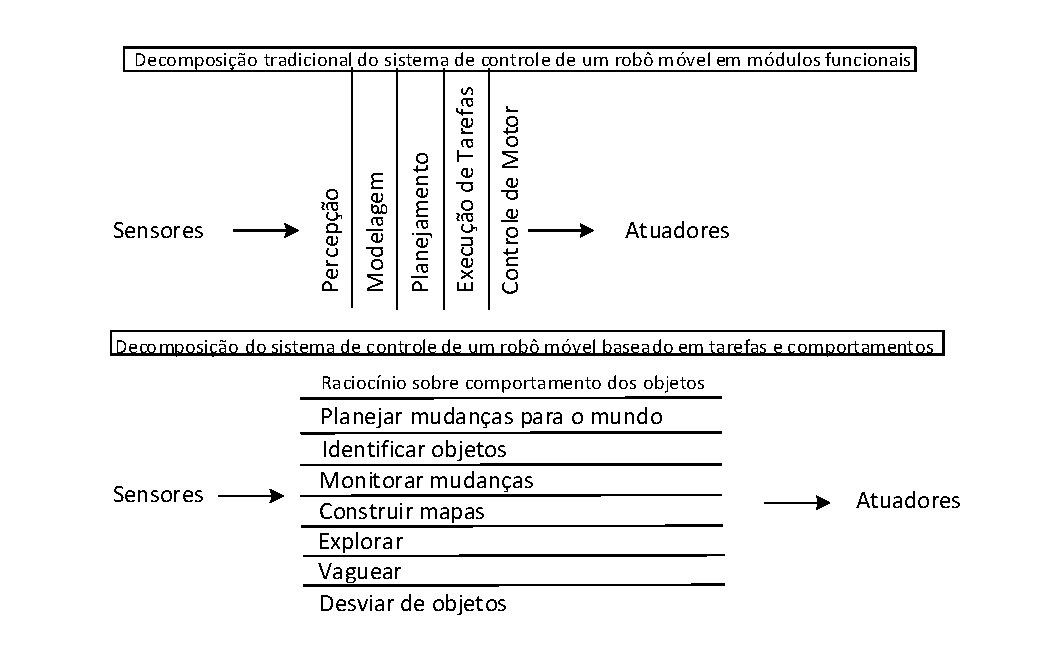
\includegraphics[width=1\columnwidth]{figs/BROOKS_1.pdf}
\caption{Arquitetura para sistema de controle de rob�s m�veis por Brooks}
\label{BROOKS_1}
\end{figure}

Na figura~\ref{BROOKS_1}, o autor define \emph{N�veis de compet�ncia}, que s�o
classes de comportamentos desejados para o rob� sobre todos os ambientes que ele
pode encontrar. As classes s�o:
\begin{enumerate}
\setcounter{enumi}{-1}
  \item Evitar contato com objetos (estacion�rios ou m�veis);
  \item Vaguear sem rumo sem bater em coisas;
  \item Explorar o ambiente vendo lugares a dist�ncia que s�o alcan��veis e
  seguir rumo em sua dire��o;
  \item Construir um mapa do ambiente e planejar trajet�rias de um lugar para
  outro;
  \item Observar mudan�as no ambiente;
  \item Raciocinar sobre o ambiente em termos de objetos identific�veis e
  realizar tarefas relacionadas a certos objetos;
  \item Formular e executar planos que envolvam mudar o estado do ambiente como
  desejado;
  \item Raciocinar sobre o comportamento de objetos no ambiente e modificar
  planos quando necess�rio;
\end{enumerate}
Vale observar que cada n�vel de compet�ncia inclui, como subconjunto, os
n�veis de compet�ncia anteriores.

Ap�s a decomposi��o na nova arquitetura, Brooks define as \emph{Camadas de
Controle}, correspondentes a cada n�vel de compet�ncia. A ideia dessa abordagem
� adicionar camadas de controle a n�veis de compet�ncias superiores sem precisar
alterar a camada do n�vel anterior. Inicia-se, portanto, com a camada de
controle para o n�vel zero de compet�ncia, ela � testada e n�o ser� mais alterada. Depois �
criada a camanda de n�vel 1, capaz de examinar os dados da camada de n�vel 0 e
injetar dados nas interfaces internas do n�vel 0, suprimindo seu tr�nsito de
dados, figura~\ref{BROOKS_2}.

\begin{figure}[H]
\centering
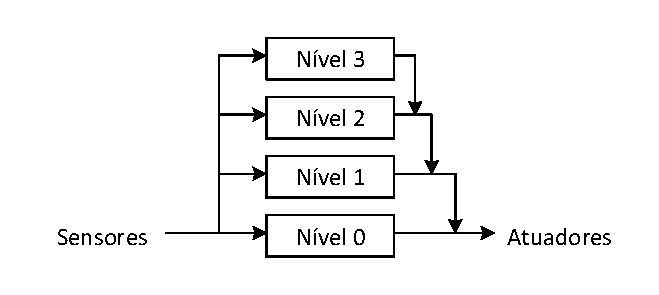
\includegraphics[width=1\columnwidth]{figs/BROOKS_2.pdf}
\caption{Camadas de controle de Brooks}
\label{BROOKS_2}
\end{figure}

Os problemas apresentados por Brooks s�o solucionados pela nova estrutura:
\begin{itemize}
  \item M�ltiplos objetivos: camadas individuais podem trabalhar em objetivos
  individuais ao mesmo tempo. Os n�veis das camadas de controle e o mecanismo de
  supress�o do tr�nsito de dados resolvem os problemas de conflito, depend�ncia
  e prioridade;
  \item M�ltiplos sensores: as camadas utilizam os dados dos sensores
  independentemente, de forma que n�o h� necessidade de se preocupar com a
  fus�o;
  \item Robustez: al�m do uso inteligente de sensores, camadas de controle de
  baixo n�vel continuam a funcionar quando novas camadas de alto n�vel s�o
  adicionadas;
  \item Extensibilidade: cada camada de controle pode possuir o seu pr�prio
  processador; 
\end{itemize}

A estrutura das camadas de controle foram constru�das por um conjunto de
pequenos processadores que enviam mensagens uns para os outros. Cada processador
� uma m�quina de estado finito. A nova arquitetura e essa nova estrutura de
camadas com eventos discretos foram a base de diversos sistemas de controle de
miss�o da atualidade. A fim de melhor o entendimento desse sistema criado por
Brooks, ser�o apresentados dois n�veis de seu controle em uma aplica��o de rob�
m�vel.

A camada de controle n�vel zero deve garantir que o rob� n�o entre em contato
com outros objetos, estacion�rios ou m�veis. Portanto, o rob� deve desviar se
algo se aproximar dele ou parar se algo estiver em sua trajet�ria. Na
figura~\ref{BROOKS_3}, podemos observar o n�vel 0 de controle do sistema.

\begin{figure}[H]
\centering
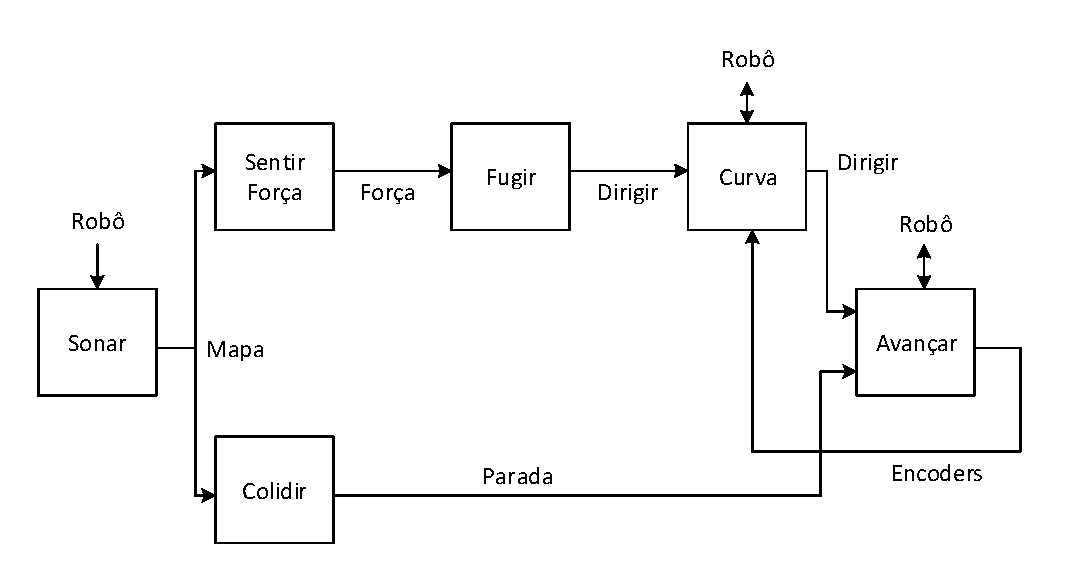
\includegraphics[width=1\columnwidth]{figs/BROOKS_3.pdf}
\caption{N�vel 0 de controle do sistema}
\label{BROOKS_3}
\end{figure}

Segue pequena descri��o de cada m�dulo:
\begin{itemize}
  \item M�dulo \emph{Curva}: comunica-se diretamente com o rob� (atuadores).
  Recebe uma mensagem \emph{Dirigir} especificando um �ngulo de giro seguido por
  uma mensagem do m�dulo \emph{Avan�o} com uma determinada magnitude. Isso faz
  com que o rob� realize uma curva e v� para o estado de \emph{Avan�o}.
  \item M�dulo \emph{Avan�o}: comando o rob� a se movimentar (atuadores), mas
  p�ra o rob� se receber mensagem do m�dulo \emph{Colis�o}. O rob� fica inativo
  e mensagens do encoder � enviado ao m�dulo \emph{Curva}, funcionando como um
  \emph{reset}, e podendo receber novos comandos.
  \item M�dulo \emph{Sonar}: recebe um vetor de informa��es de sensores do rob�,
  filtra os dados e produz um mapeamento de obst�culos para o rob� em
  coordenadas polares.
  \item M�dulo \emph{Colis�o}: monitora o mapa gerado pelo m�dulo \emph{Sonar}
  e, se detectar um obst�culo, envia um sinal de parada. Observe que este m�dulo
  funciona independentemente se o rob� est� em movimento ou parado.
  \item M�dulo \emph{Sentir For�a}: cada obst�culo detectado � somado
  como uma for�a repulsiva, gerando uma for�a resultante.
  \item M�dulo \emph{Fugir}: monitora a for�a produzida pelos obst�culos e envia
  comandos para o m�dulo \emph{Curva} se a for�a for significante.
\end{itemize}
 
 A camada de controle n�vel 1, combinada a camada de controle n�vel 0, permite
 que o rob� vagueie sem bater em obst�culos. A figura~\ref{BROOKS_3} mostra o
 sistema de controle aumentado pelo n�vel da camada 1.

\begin{figure}[H]
\centering
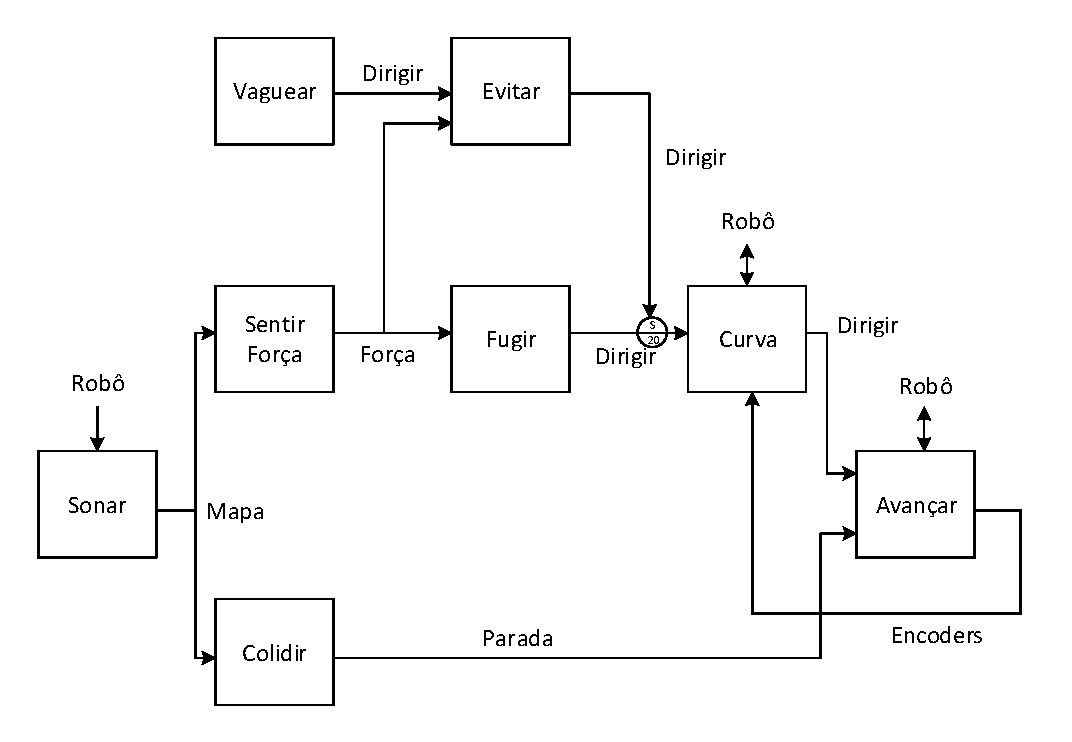
\includegraphics[width=1\columnwidth]{figs/BROOKS_4.pdf}
\caption{N�vel 0 e 1 de controle do sistema}
\label{BROOKS_4}
\end{figure}

Segue pequena descri��o de cada m�dulo:
\begin{itemize}
  \item M�dulo \emph{Vaguear}: gera nova dire��o para o rob� a cada 20 segundos.
  \item M�dulo \emph{Evitar}: recebe resultado da for�a computada pelo n�vel 0
  de controle e combina com a dire��o desejada pelo m�dulo \emph{Vaguear},
  produzindo uma nova dire��o desejada sem obst�culos. Esse resultado presume as
  computa��es do m�dulo \emph{Fugir}. Vale observar que o m�dulo \emph{Evitar}
  suprime a sa�da do m�dulo \emph{Fugir} (mecanismo de supress�o). 
\end{itemize}

A nova arquitetura de Brooks � robusta, permite intera��es din�micas, flex�vel
para integrar novas funcionalidades, f�cil para implementar e debugar, al�m de
associar sistemas de eventos discretos no controle de rob�s aut�nomos,
utilizando como m�dulos b�sicos m�quinas de estados finitos (FSM - \emph{Finite
State Machine}).
Vale ressaltar que a conex�o de diversas FSM's n�o � uma FSM e, dessa forma,
Brooks acrescentou registradores e temporizadores em suas FSM.

Antes de Brooks, em 1983, Elfes, A. [2],j� havia idealizado uma arquitetura em
m�dulos e controle distribu�do a fim de atingir efetividade em processamento
paralelo, flexibilidade de intera��o com os diversos sensores, distribuir
capacidades de decis�o e flexibilidade de expans�o e modifica��o do sistema.
Por�m o sistema de comunica��o entre m�dulos era centralizado
(\emph{Blackboard}) e s� realizavam uma determinada tarefa sob o comando de um
Plano de Controle (\emph{Control Plan}), que o usu�rio deve explicitamente
codificiar paralelismo, e os casos das exce��es e condi��es inesperadas.

Em 1989, Chatila, R.G. [3], descreve uma nova arquitetura e sistema de controle
utilizando, assim como Brooks, m�dulos de forma hier�rquica. A arquitetura do
rob� pode ser decomposta da seguinte forma:
\begin{itemize}
  \item M�dulos de sensores: processam as sa�das dos sensores. Os dados
  adquiridos por um sensor s�o processados pelo m�dulo de sensor e s�o tornados
  dispon�veis para os m�dulos de n�vel mais alto para seus pr�prios
  processamentos e interpreta��s.
  \item Unidades funcionais: realizam uma determinada fun��o no rob�. Por
  exemplo, localiza��o do rob�, combinando vis�o, odometria, laser e etc.
  \item Processos: realiza a din�mica de malha fechada entre percp��o e a��o,
  usando unidades de fun��o. O processo � representado por uma m�quina de estado
  finito, onde suas entradas s�o os dados dos m�dulos dos sensores e suas sa�das
  s�o comandos aos atuadores.
\end{itemize}
O sistema de controle de Chatila � composto por quatro componentes: Supervisor
(n�o implementado), M�dulo Executivo, Gerente de Vigil�ncia e M�dulo de
Diagn�stico (n�o implementado). Os controles funcionam como um \emph{if - then},
com diversas condi��es e a��es predeterminadas. O m�dulo de vigil�ncia �
respons�vel por:
\begin{itemize}
  \item Indicar estados dos sensores e tomar a��es de reflexo;
  \item Indica estado operacional do rob�, como n�vel da bateria;
  \item Relatar plano e estado da miss�o que est� sendo executada pelo rob�;
\end{itemize}
O m�dulo executivo fucniona como um sistema operacional. Ele recebe comandos
(miss�es) predefinidas pela interface e se comunica com o m�dulo de vigil�ncia.

Quando comparamos com Brooks, Chatila apresenta uma estrutura bem
rudimentar e l�gica simples de arquitetura e controle. Apesar de utilizar a ideia de recursos
compartilhados nos m�dulos de sensores, os automatos dos m�dulos de processo
s�o bem simplificados e dependentes de um bloco central para resolver objetivos
conflitantes.

Em 1991, em uma pesquisa financiada pelo \emph{Center for Intelligent Robotic
Systems for Space Exploration} (CIRSSE) da NASA, Wang, F.Y. [3], realizou um dos
primeiros trabalhos usando redes de Petri como m�dulos b�sicos para sistemas de
controle de miss�o, em vez de m�quinas de estados finitos (Brooks).
Alguns PNT (\emph{Petri Net Transducers}) s�o usados para traduzir os comandos
gerados pelo n�vel de organiza��o em algo compreens�vel para o n�vel de execu��o.

O sistema criado por Wang, \emph{Intelligent Mobile Robot System}(IMRS), �
baseado na teoria de intelig�ncia hier�rquica de controle, Saridis [4].
Portanto, o IMRS possui a seguinte arquitetura, FIGURA:
\begin{itemize}
  \item N�vel organizacional (organizador de tarefas): gera tarefas de
  movimenta��o de alto n�vel.
  \item N�vel de coordena��o: funciona como uma interface entre o n�vel
  organizacional e o de execu��o. O n�vel � composto por um remetente e alguns
  coordenadores. O remetente recebe o plano da tarefa do organizador, decomp�e a
  tarefa em a��es de controlee remete aos coordenadores.Os coordenadores
  traduzem os comandos de controle em instru��es de opera��o e as carrega ao
  dispositivo apropriado no n�vel de execu��o.
  \item N�vel de execu��o: executa a instru��o proveniente do n�vel de
  coordena��o reporta seus resultados a ele.
\end{itemize}
A grande contribui��o de Wang foi a utiliza��o de redes de Petri como m�dulo
b�sico de controle para seu sistema IMRS,j� que as redes de Petri foram
originalmente introduzidas para descrever as comunica��es de FSM's.
 



  \chapter{M�todo Proposto}

\section{O Algoritmo}

\begin{figure}[b]
\centering
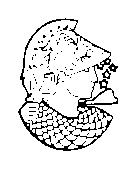
\includegraphics{minerva}
\caption{Deusa Minerva.}
\label{fig:minerva}
\end{figure}

  \chapter{Resultados e Discuss�es}

\section{Metodologia para avalia�{\~ a}o do M{\' e}todo}

\section{Valida�{\~ a}o da rotina implementada}

\subsection{Problema de autovalor padr{\~ a}o -- Caso I}

A Tabela~\ref{table:casoi} mostra as varia��es dos par�metros escolhidos para
an�lise.

\begin{table}[b]
\caption{Par{\^ a}metros do teste realizado com a matriz de Wilkinson,
3 autovalores computados.}
\label{table:casoi}
\centering
\begin{tabular}{cccc}
  \hline
  TValor de ``m'' & N$^{o}$ de itera�{\~ o}es & Tempo de CPU & Norma do Res{\' i}duo\\
  \hline
  6 & 100 & 0,09013 & $7,1474 \times 10^{-12}$\\
  10 & 28 & 0,09025 & $1,5387 \times 10^{-13}$\\
  20 & 10 & 0,100144 & $5,9011 \times 10^{-14}$\\
  40 & 6 & 0,16022 & $8,67438 \times 10^{-14}$\\
  50 & 3 & 0,24034 & $1,51537 \times 10^{-15}$\\
  \hline
\end{tabular}
\end{table}

  \chapter{Conclus�es}


  \backmatter
  \nocite{*}
  \bibliographystyle{coppe-unsrt}
  \bibliography{thesis}
  \appendix
  \chapter{C�digo Fonte}

\end{document}
